\documentclass[epsfig,10pt,fullpage]{article} 

\newcommand{\LabNum}{10}
\newcommand{\CommonDocsPath}{../../../common/docs}
\addtolength{\textwidth}{1.5in}
\addtolength{\oddsidemargin}{-0.75in}
\addtolength{\topmargin}{-0.75in}
\addtolength{\textheight}{1.5in}
\addtolength{\evensidemargin}{0.75in}
\setlength\parindent{0pt}
\raggedbottom

\usepackage{ae,aecompl}
\usepackage{epsfig,float,times}
\usepackage[hypcap]{caption}
\usepackage[pdftex, colorlinks]{hyperref}
\usepackage{graphicx}
\usepackage[usenames, dvipsnames]{color}
\usepackage{rotating}
\usepackage{tikz}
\usetikzlibrary{automata,positioning}
\usepackage{placeins}

\widowpenalty 10000
\clubpenalty 10000

\newcommand{\red}[1]{{\color{red}\sf{#1}}}
\newcommand{\green}[1]{{\color{green}\sf{#1}}}
\newcommand{\blue}[1]{{\color{blue}\sf{#1}}}
\definecolor{PineGreen}{rgb}{0.0, 0.47, 0.44}
\definecolor{ForestGreen}{rgb}{0.13, 0.55, 0.13}
\definecolor{Brown}{rgb}{0.59, 0.29, 0.0}

\newcommand{\UPDatePublished}{Oct 2021}
\newcommand{\versnum}{21.1} %version number quartus/AMP
\newcommand{\quartusname}{Quartus\textsuperscript{\textregistered} Prime}	
\newcommand{\UPTextBar}{For \quartusname{} \versnum{}}
\newcommand{\thisyear}{2021 } %for copyright
\newcommand{\company}{FPGAcademy.org}
\newcommand{\longteamname}{FPGAcademy.org}
\newcommand{\teamname}{FPGAcademy}
\newcommand{\website}{FPGAcademy.org}

\newcommand{\productAcronym}{AMP}
\newcommand{\productNameShort}{Monitor Program}

\newcommand{\productNameMedTM}{A Monitor Program}
\newcommand{\productNameMed}{A Monitor Program}

%\newcommand{\headerLogoFilePath}[1]{#1/FPGAcademy.png}

% listings is a package that supports encapsulating source code in LaTeX conveniently
\usepackage{listings}

\def\expandparam\lstinputlisting[#1]#2{\edef\tmp{\noexpand\lstinputlisting[#1]{#2}}\tmp}

%%%%%%%%%%%%%%%%%%%% Source Code Formatting %%%%%%%%%%%%%%%%%%%%
\definecolor{globalCommentColour}{rgb}{0.588,0.588,0.588}

%%%%%%%%%%%%%%%%%%%%%%%%%%%%%%%%%%%%%%%%%%%%%%%%%%%%
% Defining language style
% NiosII ASM
\lstdefinelanguage[NiosII]{Assembler} {
  morekeywords={add, addi, and, andhi, andi, beq, bge, bgeu, bgt, bgtu, ble,  bleu, blt, bltu, bne, br, break,
  bret, call, callr, cmpeq, cmpeqi, cmpge, cmpgei, cmpgeu, cmpgeui, cmpgt, cmpgti, cmpgtu, cmpgtui, cmple,
  cmplei, cmpleu, cmpleui, cmplt, cmplti, cmpltu, cmpltui, cmpne, cmpnei, custom, div, divu, eret, flushd,
  flushda, flushi, flushp, initd, initda, initi, jmp, jmpi, ldb, ldbio, ldbu, ldbuio, ldh, ldhio, ldhu, ldhuio,
  ldw, ldwio, mov, movhi, movi, movia, movui, mul, muli, mulxss, mulxsu, mulxuu, nextpc, nop, nor, or, orhi, ori,
  rdctl, rdprs, ret, rol, roli, ror, sll, slli, sra, srai, srl, srli, stb, stbio, sth, sthio, stw, stwio,
  sub, subi, sync, trap, wrctl, wrtcl, wrprs, xor, xori, xorhi, xori},
  morekeywords=[2]{.abort, .ABORT, .align, .app-file, .ascii, .asciz, .balign, .byte, .comm, .data, .def,
  .desc, .dim, .double, .eject, .else, .end, .endef, .endif, .equ, .equiv, .err, .extern, .file, .fill, .float,
  .global, .globl, .hword, .ident, .if, .include, .int, .irp, .irpc, .lcomm, .lflags, .line, .linkonce, .ln,
  .list, .long, .macro, .mri, .nolist, .octa, .org, .p2align, .psize, .quad, .rept, .sbttl, .scl, .section,
  .set, .short, .single, .size, .sleb128, .skip, .space, .stadb, .stabn, .stabs, .string, .symver, .tag,
  .text, .title, .type, .val, .uleb128, .word},
  morekeywords=[3]{et, bt, gp, sp, fp, ea, sstatus, ra, pc, status, estatus, bstatus, ienable, ipending, cpuid,
  exception, pteaddr, tlbacc, tlbmisc, eccinj, badaddr, config, mpubase, mpuacc},
  sensitive=t,
  alsoletter=.,
  morestring=[b]",
  morecomment=[s]{/*}{*/},
  morecomment=[l]\#,
}[keywords,comments,strings]
   
%% NOTE: morekeywords=[2] are GNU directives.
   
\definecolor{niosInstructionColour}{rgb}{0.000,0.608,0.000}
\definecolor{niosDirectiveColour}{rgb}{0.000,0.000,0.902}
\definecolor{niosSpecialRegColour}{rgb}{0.000,0.000,0.000}
\definecolor{niosStringColour}{rgb}{0.808,0.482,0.000}
   
%% NOTE: To make bold use: =\bfseries\color{<colour>}
\lstdefinestyle{defaultNiosStyle} {
  language=[NiosII]{Assembler},
  stringstyle=\color{niosStringColour},
  keywordstyle=\color{niosInstructionColour},
  keywordstyle=[2]\color{niosDirectiveColour},
  keywordstyle=[3]\itshape\color{niosSpecialRegColour}
}
%%%%%%%%%%%%%%%%%%%%%%%%%%%%%%%%%%%%%%%%%%%%%%%%%%%%

%%%%%%%%%%%%%%%%%%%%%%%%%%%%%%%%%%%%%%%%%%%%%%%%%%%%
% Defining language style
% ArmA9 ASM
\lstdefinelanguage[ArmA9]{Assembler} {
  morekeywords={ADC, ADD, ADDS, AND, ANDS, B, BAL, BEQ, BGE, BGT, BL, BLT, BIC, BKPT, BLX, BNE, BX, CDP, CLZ, CMN, CMP, EOR,
  EORS, LDC, LDM, LDR, LDRB, LDRBT, LDRH, LDRSB, LDRSH, LDRT, LSL, MCR, MLA, MOV, MOVW, MOVT, MRC, MRS, MSR, MUL, MVN, ORR, PLD,
  ROR, RSB, RSC, SBC, SMLAL, SMULL, STC, STM, STR, STRB, STRBT, STRH, STRT, SUB, SUBS, SWI, SWP, SWPB, TEQ, UMLAL,
  PUSH, POP, MOVS, RORS, LSR},
  morekeywords=[2]{.abort, .ABORT, .align, .app-file, .ascii, .asciz, .balign, .byte, .comm, .data, .def,
  .desc, .dim, .double, .eject, .else, .end, .endef, .endif, .equ, .equiv, .err, .extern, .file, .fill, .float,
  .global, .globl, .hword, .ident, .if, .include, .int, .irp, .irpc, .lcomm, .lflags, .line, .linkonce, .ln,
  .list, .long, .macro, .mri, .nolist, .octa, .org, .p2align, .psize, .quad, .rept, .sbttl, .scl, .section,
  .set, .short, .single, .size, .sleb128, .skip, .space, .stadb, .stabn, .stabs, .string, .symver, .tag,
  .text, .title, .type, .val, .vectors, .uleb128, .word},
  morekeywords=[3]{SP, PC, MIDR, CTR, TCMTR, TLBTR, MPIDR, ID_PFR0, ID_PFR1, ID_DFR0, ID_MMFR0, ID_MMFR1, ID_MMFR2,
  ID_MMFR3, ID_ISAR0, ID_ISAR1, ID_ISAR2, ID_ISAR3, ID_ISAR4, CCSIDR, CLIDR, AIDR, CSSELR, TTBR0, TTRB1, TTBR2, DACR,
  DFSR, IFSR, ADFSR, AIFSR, DFAAR, IFAR, ICIALLUIS, BPIALLIS, PAR, ICIALLU, ICIMVAU, BPIALL, DCIMVAC, DCISW, V2PCWPR,
  DCCVAC, DCCSW, DDIMVAC, DCISW, TLBALLIS, TLBIMVAIS, TLBIASIDIS, TLBIMVAAIS, TLBIALL, TLBIMVA, TLBIASID, TLBIMVAA,
  PMCR, PMCNTENSET, PMCNTENCLR, PMOVSR, PMSWINC, PMSELR, PMXEVTYPER, PMXEVCNTR, PMUSERENR, PMINTENSET, PMINTENCLR,
  PRRR, NRRR, PLEIDR, PLEASR, PLEFSR, PLEUAR, PLEPCR, VBAR, MVBAR, ISR, FCSEIDR, CONTEXTIDR, TPIDRURW, TPIDRURO, TPIDRPRW},
  sensitive=f,
  alsoletter=.,
  morestring=[b]",
  morecomment=[s]{/*}{*/},
  morecomment=[l]{//},
}[keywords,comments,strings]
   
%% NOTE: morekeywords=[2] are GNU directives.
   
\definecolor{armInstructionColour}{rgb}{0.000,0.608,0.000}
\definecolor{armDirectiveColour}{rgb}{0.000,0.000,0.902}
\definecolor{armSpecialRegColour}{rgb}{0.000,0.000,0.000}
\definecolor{armStringColour}{rgb}{0.808,0.482,0.000}
   
\lstdefinestyle{defaultArmStyle} {
  language=[ArmA9]{Assembler},
  stringstyle=\color{armStringColour},
  keywordstyle=\color{armInstructionColour},
  keywordstyle=[2]\color{armDirectiveColour},
  keywordstyle=[3]\itshape\color{armSpecialRegColour}
}
%%%%%%%%%%%%%%%%%%%%%%%%%%%%%%%%%%%%%%%%%%%%%%%%%%%%

%%%%%%%%%%%%%%%%%%%%%%%%%%%%%%%%%%%%%%%%%%%%%%%%%%%%
% Defining language style
% FPGAcademy ASM
\lstdefinelanguage{ASM}{
  morekeywords = [1]{mv, mvt, mvne, mvcc, add, sub, st, ld, and, b, bne, beq, bcc, bcs},
  morekeywords = [2]{word, define},
  keywordstyle = [1]\color{ForestGreen},
  keywordstyle = [2]\color{blue},
  sensitive = true,
  morecomment = [l]{//},
}

\lstset{
  language = ASM,
  basicstyle=\small\color{black}\ttfamily,
  commentstyle=\small\color{Brown}\itshape\ttfamily,
  showstringspaces=false,
  frame=none, %lines % boxed listings
  breaklines=true,
  breakatwhitespace=true,
  tabsize=3
}
%%%%%%%%%%%%%%%%%%%%%%%%%%%%%%%%%%%%%%%%%%%%%%%%%%%%

%%%%%%%%%%%%%%%%%%%%%%%%%%%%%%%%%%%%%%%%%%%%%%%%%%%%
% Defining language style
% Java
\definecolor{javaStringColour}{rgb}{0.808,0.482,0}
%%%%%%%%%%%%%%%%%%%%%%%%%%%%%%%%%%%%%%%%%%%%%%%%%%%%

%%%%%%%%%%%%%%%%%%%%%%%%%%%%%%%%%%%%%%%%%%%%%%%%%%%%
% Defining language style
% C
\definecolor{CStringColour}{rgb}{0.808,0.482,0}

\lstset{
  language = C,
  basicstyle=\small\color{black}\ttfamily, 
  commentstyle=\small\color{PineGreen}\itshape\ttfamily,
  keywordstyle=\small\color{blue}\bfseries\ttfamily,
  showstringspaces=false,
  frame=none, %lines % boxed listings
  breaklines=true,
  breakatwhitespace=true,
  tabsize=3
}
%%%%%%%%%%%%%%%%%%%%%%%%%%%%%%%%%%%%%%%%%%%%%%%%%%%%

%%%%%%%%%%%%%%%%%%%%%%%%%%%%%%%%%%%%%%%%%%%%%%%%%%%%
% Defining language style
% Verilog
\definecolor{verilogCommentColour}{rgb}{0.000,0.502,0.000}

\lstdefinestyle{defaultVerilogStyle} {
  language={Verilog},
  keywordstyle=\color{blue},
  commentstyle=\color{verilogCommentColour}
}
%%%%%%%%%%%%%%%%%%%%%%%%%%%%%%%%%%%%%%%%%%%%%%%%%%%%

%%%%%%%%%%%%%%%%%%%%%%%%%%%%%%%%%%%%%%%%%%%%%%%%%%%%
% Defining language style
% VHDL
\lstdefinestyle{defaultVHDLStyle} {
  language={VHDL},
  keywordstyle=\color{blue},
  commentstyle=\color{verilogCommentColour}
}
%%%%%%%%%%%%%%%%%%%%%%%%%%%%%%%%%%%%%%%%%%%%%%%%%%%%

%%%%%%%%%%%%%%%%%%%%%%%%%%%%%%%%%%%%%%%%%%%%%%%%%%%%
% Defining language style
% LaTeX
\lstdefinelanguage[LocalLaTeX]{TeX}[LaTeX]{TeX}{moretexcs={bf, it, sf, lstset},}

\lstdefinestyle{defaultLocalLatexStyle} {
  language=[LocalLatex]{TeX},
  keywordstyle=\color{blue}\bfseries,
  keywordstyle=[2]\color{blue},
  keywordstyle=[3]\color{blue}\bfseries
}
%%%%%%%%%%%%%%%%%%%%%%%%%%%%%%%%%%%%%%%%%%%%%%%%%%%%

%%%%%%%%%%%%%%%%%%%%%%%%%%%%%%%%%%%%%%%%%%%%%%%%%%%%
% Defining language style
% Default
\lstset{
  basicstyle=\small\color{black}\ttfamily,
  commentstyle=\small\color{globalCommentColour}\itshape\ttfamily,
  keywordstyle=\small\color{blue}\bfseries\ttfamily,
  showstringspaces=false,
  frame=none, %lines % boxed listings
  breaklines=true,
  breakatwhitespace=true,
  tabsize=3
}
%%%%%%%%%%%%%%%%%%%%%%%%%%%%%%%%%%%%%%%%%%%%%%%%%%%%


\hypersetup{
  pdftitle={Digital Logic Lab Exercise \LabNum},
  linkcolor=blue,
  hyperindex=true,
  pdfauthor={FPGAcademy.org},
  pdfkeywords={FPGAcademy.org, FPGAcademy, Lab, Exercise, Digital Logic},
  bookmarks,
  bookmarksopen=false,
  filecolor=blue,
  pdfstartview={FitH},
  urlcolor=blue,
  plainpages=false,
  pdfpagelabels=true,
  linkbordercolor={1 1 1} %no color for link border
}



\setcounter{table}{2}
\setcounter{figure}{11}

\begin{document}

\centerline{\huge Digital Logic}
~\\
\centerline{\huge Laboratory Exercise \LabNum}
~\\
\centerline{\large An Enhanced Processor}
~\\

In Laboratory Exercise 9 we described a simple processor. In
Part I of that exercise the processor itself was designed, and in Part II the processor was
connected to an external counter and a memory unit. This exercise describes subsequent
parts of the processor design. The numbering of figures and tables in this exercise 
are continued from those in Parts I and II of the preceding lab exercise.

~\\
\noindent
In this exercise we will extend the capability of the processor so that the external counter 
is no longer needed, and so that the processor can perform read and
write operations using memory or other devices. 
A schematic of the enhanced processor is given in Figure~\ref{fig:fig12}. In the figure
registers $r0$ to $r6$ are the same as in Figure~1 of Lab~1, but register $r7$ has 
been changed to a counter. This counter is used to provide the addresses in the memory from 
which the processor's instructions are read; in the preceding 
lab exercise, a counter external to the processor was used for this purpose. 
We will refer to $r7$ as the processor's {\it program counter} ({\it pc}), because this 
terminology is common for real processors available in the industry. When the processor is 
reset, {\it pc} is set to address 0. At the start of each instruction (in time step $T_0$) the 
value of {\it pc} is used as an address to read an instruction from the memory. The instruction
returned from the memory is stored into the {\it IR} register and the {\it pc} is automatically
incremented to point to the next instruction.

~\\
\noindent
The processor's control unit increments {\it pc} by using the {\it incr\_pc} signal, which is
just an enable on this counter. It is also possible to load an arbitrary address into 
{\it pc} by having the processor execute an instruction in which the destination register is 
specified as {\it pc}. In this case the control unit uses {\it r7}$_{in}$ to perform 
a {\it load} of the counter. Thus, the processor can execute instructions at any address 
in the memory, as opposed to only being able to execute instructions that are stored at 
successive addresses. The current content of {\it pc}, which always has the address of 
the {\it next} instruction to be executed, can be copied into another register if needed 
by using a {\it mv} instruction. 

~\\
\noindent
The enhanced processor will have four new instructions, which are listed
in Table~\ref{tab:new_instr}.  The {\it ld} (load) instruction {\it reads} data into 
register {\it rX} from the external memory address specified in register {\it rY}. Thus, 
the syntax [{\it rY}] means that the content of register {\it rY} is used as an
{\it external address}. The {\it st} (store) instruction {\it writes} the data contained 
in register {\it rX} into the memory address found in {\it rY}. The {\it and} instruction 
is similar to the {\it add} and {\it sub} instructions that were introduced in Lab 1.
This instruction extends the adder/subtracter unit in the processor into an
{\it arithmetic logic unit}. Besides performing addition and subtraction, it 
has the ability to generate a bit-wise logical AND (\&) of the destination register
{\it rX} with the second operand {\it Op2}. As discussed
in Lab 1, the operand {\it Op2} can be either another register {\it rY}, or immediate
data {\it \#D}.

~\\
\noindent
The {\it b\{cond\}} instruction is used to cause a processor {\it branch}, which means to
change the program counter ({\it pc}) to the address of a specific instruction. The {\it cond}
part of the branch instruction is optional and represents a {\it condition}. The instruction 
loads the constant \#{\it Label} into {\it pc} only if the specified condition evaluates to true.
An example of a condition is {\it eq}, which stands for {\it equal} (to zero). 
The instruction \texttt{beq \#Label} will load the constant {\it Label} into {\it pc} if the
last result produced by the arithmetic logic unit, which is stored in register $G$, was 0. 
The {\it b\{cond\}} instruction is discussed in more detail in Part V of this exercise.

\begin{table}[H]
\begin{center}
\begin{tabular}{l|c}
\rule[-0.075in]{0in}{0.25in}Operation & Function performed \\ \hline 
\rule[-0.075in]{0in}{0.25in}{\it ld}~~~{\it rX}, [{\it rY}] & {\it rX} $\leftarrow$ [{\it rY}] \\ 
\rule[-0.075in]{0in}{0.25in}{\it st}~~~{\it rX}, [{\it rY}] & [{\it rY}] $\leftarrow$ {\it rX} \\ 
\rule[-0.075in]{0in}{0.25in}{\it and}~~~{\it rX}, {\it Op2} & {\it rX} $\leftarrow$ {\it rX} \& {\it Op2} \\ 
\rule[-0.075in]{0in}{0.25in}{\it b\{cond\}}~~~\#{\it Label} & if ({\it cond}), {\it pc} $\leftarrow$ \#{\it Label} \\ 
\end{tabular}
\caption{New instructions in the enhanced processor.}
\label{tab:new_instr}
\end{center}
\end{table}

\begin{figure}[H]
\begin{center}
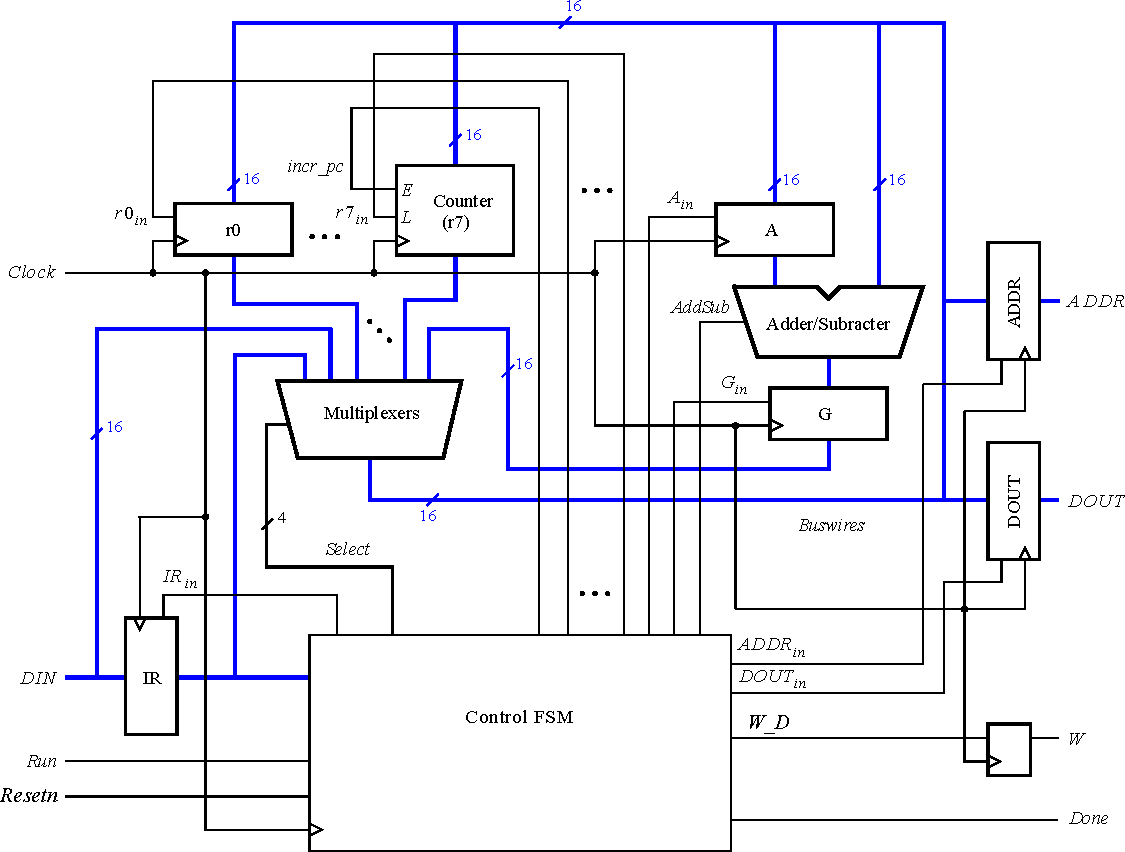
\includegraphics[scale = 0.8]{figures/figure12.pdf}
\end{center}
\caption{An enhanced version of the processor.}
\label{fig:fig12}
\end{figure}

~\\
\noindent
Recall from Lab 1 that instructions are encoded using a 16-bit format. For instructions
that specify {\it Op2} as a register the encoding is \texttt{III0XXX000000YYY}, and if {\it Op2}
is an immediate constant the format is \texttt{III1XXXDDDDDDDDD}. You should use these 
same encodings for this exercise. Assume that \texttt{III} $= 100$ for the {\it ld} instruction,
$101$ for {\it st}, $110$ for {\it and}, and $111$ for {\it b\{cond\}}.

~\\
Figure~\ref{fig:fig12} shows two registers in the processor that are used for data transfers. The 
{\it ADDR} register is used to send addresses to an external device, such as a memory module,
and the {\it DOUT} register is used by the processor to provide data that is to be stored outside 
of the processor. One use of the {\it ADDR} register is for reading, or {\it fetching}, 
instructions from memory; when the processor wants to fetch an instruction, the content
of {\it pc} is transferred across the bus and loaded into {\it ADDR}. This address is 
provided to the memory.

~\\
In addition to fetching instructions, the processor can read data 
at any address by using the {\it ADDR} register. Both data and instructions are read into 
the processor on the {\it DIN} input port.  The processor can write data for storage at 
an external address by placing this address into the {\it ADDR} register, placing the data 
to be stored into its {\it DOUT} register, and asserting the output of the {\it W} 
({\it Write}) flip-flop to 1. 

\section*{Connecting the Processor to External Devices}

Figure~\ref{fig:fig13} illustrates how the enhanced processor can be connected to memory and 
other devices. The memory unit in the figure is 16-bits wide and 256-words deep.  A diagram 
of this memory is given in Figure~\ref{fig:fig14}.
It supports both read and write operations and therefore has both address and 
data inputs, as well as a write-enable input. As depicted in Figure~\ref{fig:fig14},
the memory has a clock input that is used to store the address, data, and write enable 
inputs into registers.  This type of memory unit is called a {\it synchronous}
static random access memory (SSRAM). 

~\\
Figure~\ref{fig:fig13} also includes a 9-bit output port (register) that can be used to store 
data from the processor. In the figure this output port is connected to a set of LEDs, like 
the ones available on the DE1-SoC board. To allow the processor to select either the memory 
unit or output port when performing a write operation, the circuit includes {\it address decoding},
which is done using NOR gates and AND gates. 
If the processor's upper address lines $A_{15} A_{14} A_{13} A_{12} = 0000$, then the memory unit 
can be written. Figure~\ref{fig:fig13} shows $n$ {\it lower} address lines connected from the 
processor to the memory; since the memory has 256 words, then $n = 8$ and the memory's 
{\it address} port is driven by the processor address lines $A_7 \ldots A_0$. For
addresses in which $A_{15} A_{14} A_{13} A_{12} = 0001$, the data written by the processor
is loaded into the output port connected to {\it LEDs} in Figure~\ref{fig:fig13}.
~\\
\begin{figure}[H]
\begin{center}
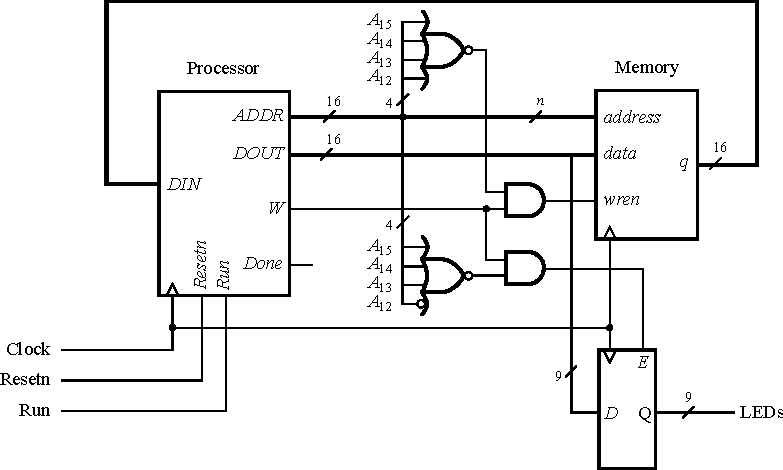
\includegraphics{figures/figure13.pdf}
\end{center}
\vspace{-0.5cm}
\caption{Connecting the enhanced processor to a memory unit and output register.}
\label{fig:fig13}
\end{figure}

\begin{figure}[b]
\begin{center}
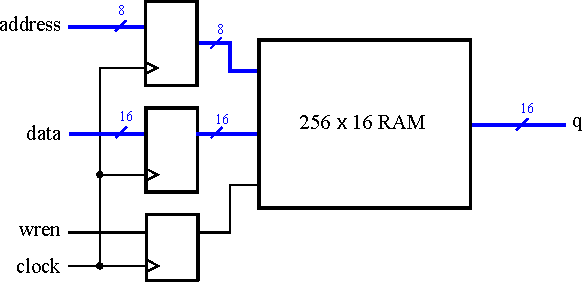
\includegraphics{figures/figure14.pdf}
\end{center}
\vspace{-0.5cm}
\caption{The synchronous SRAM unit.}
\label{fig:fig14}
\end{figure}

\section*{Part III}

Figure~\ref{fig:top} gives Verilog code for a top-level file that you can use for this
part of the exercise. The input and output ports for this module are chosen so that it can
be implemented on a DE1-SoC board. The Verilog code corresponds to the circuit 
in Figure~\ref{fig:fig13},
plus an additional input port that is connected to switches {\it SW}$_8$ $\ldots$ {\it SW}$_0$.
This input port can be read by the processor at addresses in which $A_{15} \ldots A_{12} = 0011$.
(Switch {\it SW}$_9$ is not a part of the input port, because it is dedicated for use as the
processor's {\it Run} input.) To support reading from both the SW input port and the memory
unit, the top-level circuit includes a multiplexer that feeds the processor's {\it DIN}
input. This multiplexer is described by using an \texttt{if-else} statement inside 
the \texttt{always} block in Figure~\ref{fig:top}.

~\\
\noindent
The code in Figure~\ref{fig:top} is provided with this exercise, along with a few
other source-code files: {\it flipflop.v}, {\it inst\_mem.v}, {\it inst\_mem.mif}, and 
(part of) {\it proc.v}. The {\it inst\_mem.v} source-code file was created by using the Quartus IP 
Catalog to instantiate a \texttt{RAM:1-PORT} memory module. It has a 16-bit wide read/write
data port and is 256-words deep, corresponding to Figure~\ref{fig:fig14}.

~\\
\noindent
The Verilog code in the {\it proc.v} file implements register {\it r7} as a program counter,
as discussed above, and includes a number of changes that are needed to support the 
new {\it ld}, {\it st}, {\it and}, and {\it b\{cond\}} instructions. In this part you are to 
augment this Verilog code to complete the implementation of the {\it ld} and
{\it st} instructions, as well as the {\it and} instruction. You do not 
need to work on the {\it b\{cond\}} instruction for this part. 

\lstset{language=Verilog,numbers=none,escapechar=|}
\begin{figure}[h]
\begin{center}
\begin{minipage}[h]{15 cm}
\begin{lstlisting}[name=proc]
|\label{line:module}|module part3 (KEY, SW, CLOCK_50, LEDR);
	input [0:0] KEY;
	input [9:0] SW;
	input CLOCK_50;
	output [9:0] LEDR;	

	wire [15:0] DOUT, ADDR;
	wire Done, W;
	reg [15:0] DIN;
	wire inst_mem_cs, SW_cs, LED_reg_cs;
	wire [15:0] inst_mem_q;
	wire [8:0] LED_reg, SW_reg;      // LED[9] and SW[9] are used for Run

   proc U3 (DIN, KEY[0], CLOCK_50, SW[9], DOUT, ADDR, W, Done);

	assign inst_mem_cs = (ADDR[15:12] == 4'h0);
	assign LED_reg_cs = (ADDR[15:12] == 4'h1);
	assign SW_cs = (ADDR[15:12] == 4'h3);
	inst_mem U4 (ADDR[7:0], CLOCK_50, DOUT, inst_mem_cs & W, inst_mem_q);

	always @ (*)                     // input multiplexer
	   if (inst_mem_cs == 1'b1)
		   DIN = inst_mem_q;
	   else if (SW_cs == 1'b1)
		   DIN = {7'b0000000, SW_reg};
	   else
		   DIN = 16'bxxxxxxxxxxxxxxxx;

	regn #(.n(9)) U5 (DOUT[8:0], LED_reg_cs & W, CLOCK_50, LED_reg);
	assign LEDR[8:0] = LED_reg;
   assign LEDR[9] = SW[9];

	regn #(.n(9)) U7 (SW[8:0], 1'b1, CLOCK_50, SW_reg); // SW[9] is used for Run
endmodule
\end{lstlisting}
\end{minipage}
\caption{Verilog code for the top-level file.}
\label{fig:top}
\end{center}
\end{figure}

\newpage
\noindent
Perform the following:
\begin{enumerate}
\item Extend the code in {\it proc.v} so that the enhanced processor fully implements the 
{\it ld}, {\it st}, and {\it and} instructions. Test your Verilog code by using the ModelSim
simulator. Sample setup files for ModelSim, including a testbench, are provided along with 
the other files for this exercise.  The sample testbench first resets the processor system
and then asserts the {\it Run} switch, {\it SW}$_9$, to 1. A sample program to test your 
processor is also provided, in a file called {\it inst\_mem.mif}. This file represents the 
assembly-language program shown in Figure~\ref{fig:assembly}, which tests 
the {\it ld} and {\it st} instructions by reading the values of the SW switches and writing 
these values to the LEDs, in an endless loop. At the beginning of a simulation, ModelSim loads 
the contents of the file {\it inst\_mem.mif} into the {\it inst\_mem} memory module, so
that the program can be executed by the processor.  Examine the signals inside 
your processor, as well as the external LEDR values, as the program executes within the
ModelSim simulation.

An {\it assembler} software tool, called {\it sbasm.py}, can be used with your processor.
The Assembler is written in Python and is available at
\texttt{https://github.com/profbrown/sbasm.git}. To use this 
Assembler you have to first install Python (version 3) on your computer. The Assembler includes
a README file that explains how to install and use it. The {\it sbasm.py} Assembler can 
generate machine code for all of the processor's instructions. The provided file 
{\it inst\_mem.mif} was created by using {\it sbasm.py} to {\it assemble} the program in 
Figure~\ref{fig:assembly}. As the figure indicates, you can define symbolic
constants in your code by using the .\blue{define} {\it directive}, and you can use 
labels to refers to lines of code, such as \texttt{MAIN}.
Comments are specified in the code by using \texttt{//}. The assembler ignores anything 
on a line following \texttt{//}.

\lstset{language=ASM,numbers=none,escapechar=|}
\begin{figure}[H]
\begin{center}
\begin{minipage}[h]{12.5 cm}
\begin{lstlisting}[name=proc]
|\label{line:module}|.define LED_ADDRESS 0x1000
.define SW_ADDRESS 0x3000

// Read SW switches and display on LEDs
			mvt	r3, #LED_ADDRESS	// point to LED port
			mvt	r4, #SW_ADDRESS	// point to SW port
MAIN:		ld		r0, [r4]				// read SW values
			st		r0, [r3]				// light up LEDs
			mv 	pc, #MAIN
\end{lstlisting}
\end{minipage}
\caption{Assembly-language program that uses {\it ld} and {\it st} instructions.}
\label{fig:assembly}
\end{center}
\end{figure}

An example result produced by using {\it ModelSim} for a correctly-designed circuit 
is given in Figure~\ref{fig:part3}. It shows the execution of the first four instructions
in Figure~\ref{fig:assembly}.

\item Once your simulation results are correct, use the Quartus Prime software to implement your
Verilog code on a DE1-SoC board. A sample Quartus project file, {\it part3.qpf}, and Quartus
settings file, {\it part3.qsf}, are provided with the exercise. Compile your code using the 
Quartus software, and download the resulting circuit 
into the DE1-SoC board. Toggle the SW switches and observe the LEDs to test your circuit.
\end{enumerate}

\begin{figure}[H]
	\begin{center}
		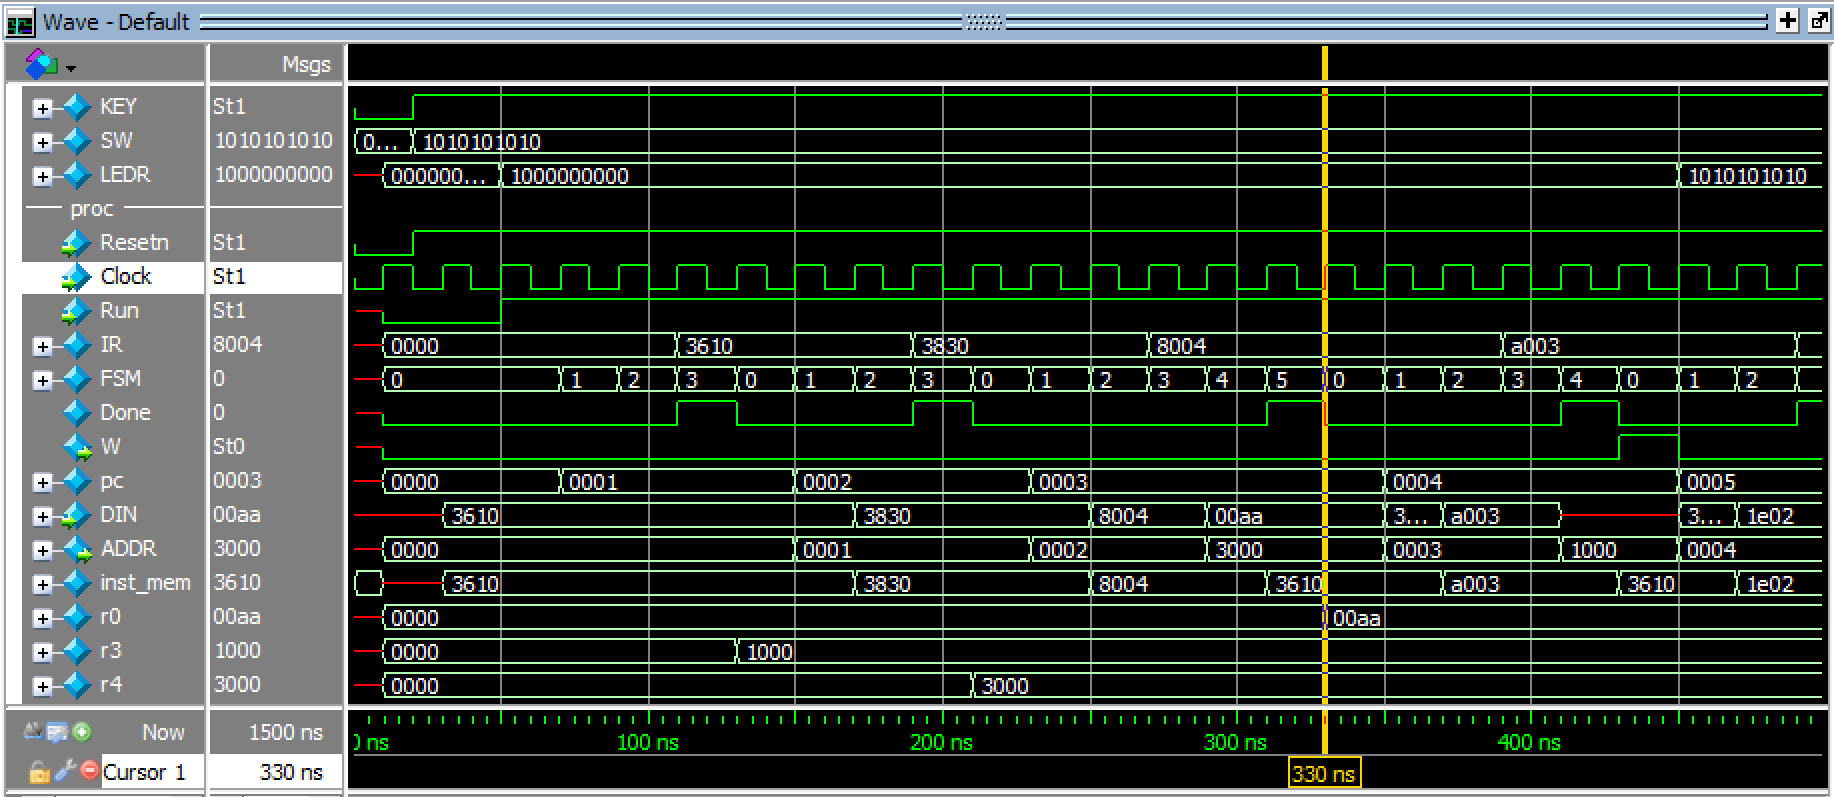
\includegraphics[width=\textwidth]{figures/part3.png}
	\end{center}
	\caption{Simulation results for the processor.}
	\label{fig:part3}
\end{figure}

\section*{Part IV}
In this part you are to create a new Verilog module that represents an output port called 
{\it seg7}. It will allow your processor to write data to each of the six 7-segment displays on a 
DE1-SoC board. The {\it seg7} module will include six write-only seven-bit registers,
one for each display. Each register should directly drive the segment lights for one 
seven-segment display, so that the processor can write characters onto the displays. 

~\\
\noindent
Perform the following:

\begin{enumerate}
\item A top-level file is provided for this part
called {\it part4.v}. The top-level module has output ports for connecting
to each of the 7-segment displays. 
Pin assignments for these ports, which are called {\it HEX0}[6:0], {\it HEX1}[6:0], 
$\ldots$, {\it HEX6}[6:0], are included in the Quartus settings file {\it part4.qsf}. 
For each display, segment 0 is on the top of the display, and then segments 1 to 5 are assigned
in a clockwise fashion, with segment 6 being in the middle of the display.

The {\it part4.v} Verilog code includes address decoding for the new {\it seg7} module, 
so that processor addresses in which $A_{15} A_{14} A_{13} A_{12} = 0010$ select this module.
The intent is that address \texttt{0x2000} should write to the register that controls 
display {\it HEX0}, \texttt{0x2001} should select the register for {\it HEX1}, and 
so on. For example, if your processor 
writes \texttt{0} to address \texttt{0x2000}, then the {\it seg7} module
should turn off all of the segment-lights in the {\it HEX0} display; writing \texttt{0x7f} 
should turn on all of the lights in this display. 

\item 
You are to complete the partially-written Verilog code in the file {\it seg7.v}, so that
it contains the required six registers---one for each 7-segment display. 
        
\item You can compile and test your Verilog code by using the ModelSim setup files that 
are provided for this part of the exercise. An {\it inst\_mem.mif} file is also provided
that corresponds to the assembly-language program shown in 
Figure~\ref{fig:7segs}. This program works as follows: it reads the {\it SW} switch port and 
lights up a seven-segment display corresponding to the value read on {\it SW}$_{2-0}$. For
example, if {\it SW}$_{2-0} = 000$, then the digit~\texttt{\red{0}} is shown on {\it HEX0}.
If {\it SW}$_{2-0} = 001$, then the digit~\texttt{\red{1}} is displayed on {\it HEX1}, 
and so on, up to the digit~\texttt{\red{5}} which would be shown on {\it HEX5} if
{\it SW}$_{2-0} = 101$.

\item Once your simulation results look correct, you should compile the provided Quartus
project, and then download and test the circuit on a DE1-SoC board.
\end{enumerate}

\lstset{language=ASM,numbers=none,escapechar=|}
\begin{figure}[H]
\begin{center}
\begin{minipage}[h]{15 cm}
\begin{lstlisting}[name=proc]
|\label{line:module}|
.define HEX_ADDRESS 0x2000
.define SW_ADDRESS 0x3000

// This program shows the digits 543210 on the HEX displays. Each digit has to
// be selected by using the SW switches.
			mv		r5, pc				// return address for subroutine
			mv 	pc, #BLANK			// call subroutine to blank the HEX displays
MAIN:		mvt	r2, #HEX_ADDRESS	// point to HEX port
			mv 	r3, #DATA			// used to get 7-segment display pattern

			mvt	r4, #SW_ADDRESS	// point to SW port
			ld		r0, [r4]				// read switches
			and   r0, #0x7          // use only SW2-0
			add	r2, r0				// point to correct HEX display
			add	r3, r0				// point to correct 7-segment pattern

			ld		r0, [r3]				// load the 7-segment pattern
			st		r0, [r2]				// light up HEX display

			mv 	pc, #MAIN

// subroutine BLANK
// 	This subroutine clears all of the HEX displays
//	input: none
//	returns: nothing
// changes: r0 and r1. Register r5 provides the return address
BLANK:   mv 	r0, #0				// used for clearing
			mvt	r1, #HEX_ADDRESS	// point to HEX displays
			st		r0, [r1]				// clear HEX0
			add	r1, #1
			st		r0, [r1]				// clear HEX1
			add	r1, #1
			st		r0, [r1]				// clear HEX2
			add	r1, #1
			st		r0, [r1]				// clear HEX3
			add	r1, #1
			st		r0, [r1]				// clear HEX4
			add	r1, #1
			st		r0, [r1]				// clear HEX5

			add	r5, #1
			mv		pc, r5				// return from subroutine

DATA:		.word 0b00111111			// '0'
			.word 0b00000110			// '1'
			.word 0b01011011			// '2'
			.word 0b01001111			// '3'
			.word 0b01100110			// '4'
			.word 0b01101101			// '5'
\end{lstlisting}
\end{minipage}
\caption{Assembly-language program that tests the seven-segment displays.}
\label{fig:7segs}
\end{center}
\end{figure}

\section*{Part V}
In this part you are to enhance your processor so that it implements the {\it b\{cond\}}
instruction.  The {\it conditions} supported by the processor are called 
{\it eq}, {\it ne}, {\it cc}, and {\it cs}, which means that the variations of the branch
instruction are {\it b}, {\it beq}, {\it bne}, {\it bcc}, and {\it bcs}. The {\it b}
instruction {\it always} branches. For example, \texttt{b \#MAIN} loads the address
\texttt{MAIN} into the program counter. The meanings of the conditional versions are 
explained below.

~\\
\noindent
The instruction {\it beq} means {\it branch if equal} (to zero). This instruction performs
a branch operation (i.e., loads the provided \texttt{\#LABEL} into the program counter) if the 
most recent result of an instruction executed using the
arithmetic logic unit (ALU), which is stored in register $G$, was~0. 
Similarly, {\it bne} means {\it branch if not
equal} (to zero).  It performs a branch only if the contents of $G$ are not equal to 0.
The instruction {\it bcc} stands for {\it branch if carry clear}. It branches if the last
add/subtract operation did {\it not} produce a carry-out. The opposite branch condition, 
{\it bcs}, {\it branch if carry set}, performs a branch if the most recent add/sub
generated a carry-out. To support the conditional branch instructions, you should 
create two {\it condition-code flags} in your processor. One flag, {\it z}, should have
the value 1 when the ALU generates a result of zero; otherwise {\it z} should be 0. The other 
flag, {\it c}, should be 1 when the adder/subtracter in the ALU produces a carry-out;
otherwise {\it c} should be 0. Thus, {\it c} should be 1 when an {\it add} 
instruction generates a carry-out,
or when a {\it sub} operation requires a borrow for the most-significant bit. Your FSM
controller should examine these flags in the appropriate clock cycles when executing the 
{\it b\{cond\}} instructions.

~\\
\noindent
The branch instructions are encoded using the format \texttt{III1XXXDDDDDDDDD}, where
\texttt{DDDDDDDDD} is the branch address and \texttt{XXX} is the branch condition. Assume
that conditions are encoded as {\it none} (always branch) $= 000$, {\it eq}~$= 001$,
{\it ne} $= 010$, {\it cc} $= 011$, and {\it cs} $= 100$.

~\\
\noindent
Perform the following:

\begin{enumerate}
\item 
Enhance your processor so that it implements the condition-code flags {\it z} and {\it c},
and supports the {\it b\{cond\}} instruction. 
To help with testing and debugging of your processor, setup files for ModelSim are provided, 
including a testbench. It simulates your processor instantiated in the top-level file
{\it part5.v}, which is the same as the one from Part IV. 
An example {\it inst\_mem.mif} file is also provided, which corresponds 
to the program in Figure~\ref{fig:branches}. This program is quite short, 
which makes it suitable for visual inspection of the waveforms produced by a ModelSim simulation. 
The program uses a sequence of instructions that test the various conditional branches. 
If the program reaches the line of code labelled \texttt{DEAD}, then at least one 
instruction has not worked properly. An example of ModelSim output for a correctly-working
processor is given in Figure~\ref{fig:part4}. It shows the processor executing instructions
near the end of the code in Figure~\ref{fig:branches}. The instruction that is completed
at simulation time 1030 ns is \texttt{add r0, \#1} (\texttt{0x5001}). As shown in the figure,
this instruction causes the carry flag, {\it c}, to become 1. The next instruction loaded
into {\it IR}, at time 1090 ns, is \texttt{bcs \#0xC} (\texttt{0xF80C}). Finally, the
instruction loaded at 1170~ns is \texttt{b~\#0} (\texttt{0xF000}). 

\lstset{language=ASM,numbers=none,escapechar=|}
\begin{figure}[H]
\begin{center}
\begin{minipage}[h]{13.5 cm}
\begin{lstlisting}[name=proc]
MAIN:    mv    r0, #2
LOOP: 	sub   r0, #1        // subtract to test bne
			bne   #LOOP
			beq   #T1           // r0 == 0, test beq
			mv    pc, #DEAD
T1:      mvt   r0, #0xFF00
         add   r0, #0xFF     // r0 = 0xFFFF
			bcc   #T2           // carry = 0, test bcc
			mv    pc, #DEAD
T2:      add   r0, #1
			bcs   #T3           // carry = 1, test bcs
			mv    pc, #DEAD
T3:	   b     #MAIN
DEAD:    mv    pc, #DEAD
\end{lstlisting}
\end{minipage}
\caption{Assembly-language program that uses various branches.}
\label{fig:branches}
\end{center}
\end{figure}

\begin{figure}[H]
	\begin{center}
		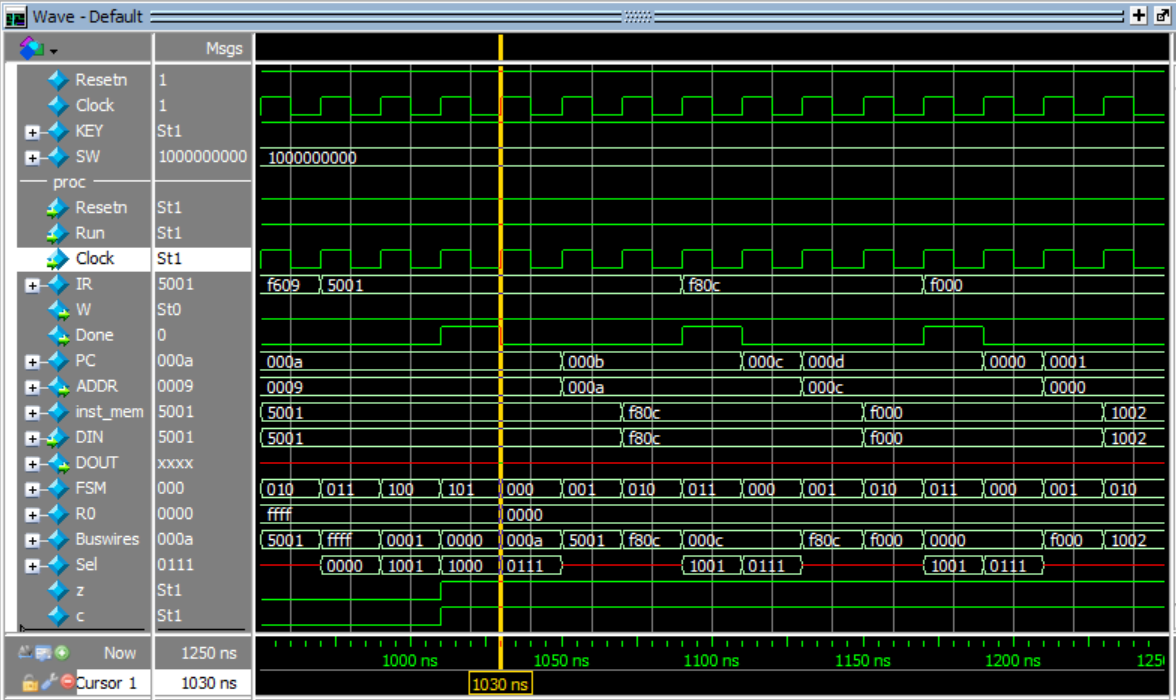
\includegraphics[width=\textwidth]{figures/part5.png}
	\end{center}
	\caption{Simulation results for the processor.}
	\label{fig:part4}
\end{figure}

\item Once your ModelSim simulation indicates a correctly-functioning processor you should
implement it on a DE1-SoC board.  A Quartus project file {\it part5.qpf} and settings file
{\it part5.qsf} are provided for this purpose. To test your processor, you can use the 
assembly-language program displayed in Figure~\ref{fig:sitbooboosit}. It provides code that
tests for the correct operation of instructions supported by the enhanced processor. 
If all of the tests pass, then
the program shows the word \texttt{\red{PASSEd}} on the seven-segment displays. It also shows 
a binary value on the LEDs that represents the number of successful tests performed. If any test
fails, then the program shows the word \texttt{\red{FAILEd}} on the seven-segment displays and 
places on the LEDs the address in the memory of the instruction that caused the failure.
Assemble the program, which is provided in a file called {\it sitbooboosit.s}, by using 
the {\it sbasm.py} assembler.
        
Use the output produced by {\it sbasm.py} to {\it overwrite} the file {\it inst\_mem.mif}
that you used in the beginning of this part of the exercise to simulate your processor
system with ModelSim. Open the Quartus software, compile the {\it part5} project, 
and download it onto 
your DE1-SoC board.  If the {\it Run} signal is asserted, then your processor should execute the 
{\it sitbooboosit} program. If a failure is encountered, then the 
offending instruction can be identified by cross-referencing the LED pattern with the addresses
in the file {\it inst\_mem.mif}.
\end{enumerate}

\vspace{-0.5cm}
\lstset{language=ASM,numbers=none,escapechar=|}
\begin{figure}[H]
\begin{center}
\begin{minipage}[h]{14 cm}
\begin{lstlisting}[name=proc]
.define LED_ADDRESS 0x1000
.define HEX_ADDRESS 0x2000
			mv 	r2, #0		// used to count number of successful tests
			mv 	r6, #T1		// save address of next test
			sub	r0, r0		// set the z flag
T1:		bne	#FAIL    	// test bne; should not take the branch!
			mv 	r6, #C1		// save address of next test
C1:      beq   #C2         // test beq; should take the branch
    		b	   #FAIL    	// Argh!
C2:		add	r2, #2		// count the last two successful tests
\end{lstlisting}
\end{minipage}
\caption{Assembly-language program that tests various instructions. (Part $a$)}
\label{fig:sitbooboosit}
\end{center}
\end{figure}

\begin{center}
\begin{minipage}[t]{14 cm}
\begin{lstlisting}[name=proc]
			mv		r6, #T2			// save address of next test
T2:		bne	#S1    			// test bne; should take the branch!
			mv		pc, #FAIL
S1:		mv 	r6, #C3			// save address of next test
C3:      beq   #FAIL          // test beq; should not take the branch
			add	r2, #2			// count the last two successful tests

			mv		r6, #T3			// save address of next test
			mv		r3, #ALLONES
			ld		r3, [r3]
			add	r3, #1			// set the c flag

T3:		bcc	#FAIL    		// test bcc; should not take the branch!
			mv 	r6, #C4			// save address of next test
C4:      bcs   #C5            // test bcs; should take the branch
    		b	   #FAIL    		// Argh!
C5:		add	r2, #2			// count the last two successful tests

			mv		r6, #T4
			mv		r3, #0
			add	r3, r3			// clear carry flag

T4:		bcc	#S2   			// test bcc; should take the branch!
			mv		pc, #FAIL
S2:		mv 	r6, #C6			// save address of next test
C6:      bcs   #FAIL          // test bcs; should bot take the branch!
         add	r2, #2			// count the last two successes

// finally, test ld and st from/to memory
			mv		r6, #T5			// save address of next test
			mv		r4, #_LDTEST
			ld		r4, [r4]
			mv		r3, #0x1A5
			sub	r3, r4
T5:		bne	#FAIL	      	// should not take the branch!
			add	r2, #1			// increment success count

			mv		r6, #T6			// save address of next test
			mv		r3, #0x1A5
			mv		r4, #_STTEST
			st		r3, [r4]		
			ld		r4, [r4]
			sub	r3, r4
T6:		bne	#FAIL    		// should not take the branch!
			add	r2, #1			// increment success count

			mv		pc, #PASS
			// Loop over the six HEX displays
FAIL:		mvt	r3, #LED_ADDRESS
			st		r6, [r3]			// show address of failed test on LEDs
			mv		r5, #_FAIL
			mv		pc, #PRINT
PASS:		mvt	r3, #LED_ADDRESS
			st		r2, [r3]			// show success count on LEDs
			mv		r5, #_PASS
\end{lstlisting}
\end{minipage}
\end{center}

\begin{center}
Figure \ref{fig:sitbooboosit}: Assembly-language program that tests various instructions. (Part $b$)
\end{center}

\begin{center}
\begin{minipage}[t]{12.5 cm}
\begin{lstlisting}[name=proc]
PRINT:	mvt	r4, #HEX_ADDRESS		// address of HEX0 
			// We would normally use a loop counting down from 6
			// with bne to display the six letters. But in this
			// testing code we can't assume that bne even works!

			ld		r3, [r5]			// get letter 
 			st		r3, [r4]			// send to HEX display
 			add	r5, #1			// ++increment character pointer 
 			add	r4, #1			// point to next HEX display
			ld		r3, [r5]			// get letter 
 			st		r3, [r4]			// send to HEX display
 			add	r5, #1			// ++increment character pointer 
 			add	r4, #1			// point to next HEX display
			ld		r3, [r5]			// get letter 
 			st		r3, [r4]			// send to HEX display
 			add	r5, #1			// ++increment character pointer 
 			add	r4, #1			// point to next HEX display
			ld		r3, [r5]			// get letter 
 			st		r3, [r4]			// send to HEX display
 			add	r5, #1			// ++increment character pointer 
 			add	r4, #1			// point to next HEX display
			ld		r3, [r5]			// get letter 
 			st		r3, [r4]			// send to HEX display
 			add	r5, #1			// ++increment character pointer 
 			add	r4, #1			// point to next HEX display
			ld		r3, [r5]			// get letter 
 			st		r3, [r4]			// send to HEX display
 			add	r5, #1			// ++increment character pointer 
 			add	r4, #1			// point to next HEX display
			
HERE:		mv		pc, #HERE

_PASS:	.word	0b0000000001011110	// d
			.word	0b0000000001111001	// E
			.word	0b0000000001101101	// S
			.word	0b0000000001101101	// S
			.word	0b0000000001110111	// A
			.word 0b0000000001110011	// P

_FAIL:	.word	0b0000000001011110	// d
			.word	0b0000000001111001	// E
			.word	0b0000000000111000	// L
			.word	0b0000000000110000	// I
			.word	0b0000000001110111	// A
			.word 0b0000000001110001	// F

ALLONES:	.word 0xFFFF
_LDTEST:	.word 0x1A5
_STTEST:	.word 0x15A
\end{lstlisting}
\end{minipage}
\end{center}

\begin{center}
Figure \ref{fig:sitbooboosit}: Assembly-language program that tests various instructions. (Part $c$)
\end{center}

\section*{Part VI}
Write an assembly-language program that displays a binary counter on the LED port. Initialize 
the counter to 0, and then increment the counter by one in an endless loop. You should be
able to control the speed at which the counter is incremented by using nested delay loops, 
along with the SW switches. If the SW switches are set to their maximum value, 
\texttt{0b111111111}, then the delay loops should cause the counter to increment slowly enough 
so that each change in the counter can be visually observed on the LEDs. Lowering the value 
of the SW switches should make the counter increment more quickly up to some maximum speed. 

~\\
\noindent
You can assemble your program by using the {\it sbasm.py} assembler, and then run it on
your processor system from Part V. To do this, use the output produced by {\it sbasm.py} to 
{\it overwrite} the file {\it inst\_mem.mif} in the folder that holds your Quartus project for
Part V. To make use of the new {\it inst\_mem.mif} file you do not need to completely 
recompile your Verilog code from Part V. Instead, execute the Quartus command 
\texttt{Processing} $>$ \texttt{Update Memory Initialization File}, to include the 
new {\it inst\_mem.mif} file in your Quartus project. Next, select the Quartus 
command \texttt{Processing} $>$ \texttt{Start} $>$ \texttt{Start Assembler} to produce a new 
programming {\it bitstream} for your DE1-SoC board. Finally, use the Quartus Programmer to 
download the new bitstream onto your board. If the {\it Run} signal is asserted, your
processor should execute the new program.

\section*{Part VII}
Augment your assembly-language program from Part VI so that counter values are displayed
on the seven-segment display port rather than on the LED port. You should display the
counter values as decimal numbers from \texttt{\red{0}} to \texttt{\red{65535}}.
The speed of counting should be controllable using the SW switches in the same way as for
Part VI. As part of your solution you may want to make use of the code shown in 
Figure~\ref{fig:div10}. This code provides a subroutine that divides the number in
register $r0$ by 10, returning the quotient in $r1$ and the remainder in $r0$. Dividing by 10 is a 
useful operation when performing binary-to-decimal conversion. The \texttt{DIV10} subroutine
assumes that $r6$ is set up to be used as a {\it stack pointer}. Register $r2$ is saved on the
stack at the beginning of the subroutine, and then restored before returning. This is done so
that $r2$ is not unnecessarily changed by the subroutine. A skeleton of the required code
for this part is shown in Figure~\ref{fig:part7}.

\lstset{language=ASM,numbers=none,escapechar=|}
\begin{figure}[H]
\begin{center}
\begin{minipage}[h]{15 cm}
\begin{lstlisting}[name=proc]
// subroutine DIV10
//	  This subroutine divides the number in r0 by 10
//	  The algorithm subtracts 10 from r0 until r0 < 10, and keeps count in r1
//	  This subroutine assumes that r6 can be used as a stack pointer
//	  input: r0
//	  returns: quotient Q in r1, remainder R in r0
DIV10:
			sub	r6, #1				// save registers that are modified
			st		r2, [r6]				// save on the stack

			mv 	r1, #0				// init Q
DLOOP:	mv 	r2, #9				// check if r0 is < 10  yet
			sub	r2, r0
			bcc	#RETDIV				// if so, then return

INC:		add	r1, #1				// but if not, then increment Q
			sub	r0, #10				// r0 -= 10
			b 		#DLOOP				// continue loop
RETDIV:
			ld		r2, [r6]				// restore from the stack
			add	r6, #1
			add	r5, #1				// adjust the return address
			mv		pc, r5				// return results
\end{lstlisting}
\end{minipage}
\caption{A subroutine that divides by 10}
\label{fig:div10}
\end{center}
\end{figure}

\noindent
As described previously, assemble your program with {\it sbasm.py}, update your {\it MIF} file 
in the Quartus software, generate a new bitstream file by using the Quartus Assembler, and 
then download the new bitstream onto your DE1-SoC board to run your new program. 

\lstset{language=ASM,numbers=none,escapechar=|}
\begin{figure}[H]
\begin{center}
\begin{minipage}[h]{15 cm}
\begin{lstlisting}[name=proc]
.define HEX_ADDRESS 0x2000
.define SW_ADDRESS 0x3000
.define STACK 256						// bottom of memory

// This program shows a decimal counter on the HEX displays
			mv 	r6, #STACK			// stack pointer
			mv		r5, pc				// return address for subroutine
			mv 	pc, #BLANK			// call subroutine to blank the HEX displays
MAIN:		mv 	r0, #0				// initialize counter
LOOP:		mvt	r1, #HEX_ADDRESS	// point to HEX port
			...
         ... use a loop to extract and display each digit
         ...

// Delay loop for controlling the rate at which the HEX displays are updated
         ...
         ... read from SW switches, and use a nested delay loop
         ...

			add	r0, #1				// counter += 1
			bcc	#LOOP					// continue until counter overflows

			mv		r5, pc				// return address for subroutine
			mv 	pc, #BLANK			// call subroutine to blank the HEX displays
			b 	   #MAIN

// subroutine DIV
         ...
         ... code not shown here
         ...
			add	r5, #1				// adjust the return address
			mv		pc, r5				// return results

// subroutine BLANK
         ...
         ... code not shown here
         ...
			add	r5, #1
			mv		pc, r5				// return from subroutine

DATA:		.word 0b00111111			// '0'
			....
\end{lstlisting}
\end{minipage}
\caption{Skeleton code for displaying decimal digits.}
\label{fig:part7}
\end{center}
\end{figure}

\end{document}
